% Niveau :      PCSI *
% Discipline :  Méca
% Mots clés :   Ballistique, Mécanique du point, PFD, Chute libre

\begin{exercise}{Le bûcheron canadien}{2}{Sup, Spé}
{Mécanique,Moment cinétique}{bermu}

Un bûcheron canadien veut abattre un pin qui est légèrement incliné suite à une tempête. On assimile cet arbre à une tige longue et homogène de longueur $L$ et de masse $m$. Alors qu'il scie l'arbre à la base du tronc, l'arbre se met à tomber s'appuyant sur la base de la souche, supposée fixe lors de la chute.

On appelle $\theta$ l'inclinaison de l'arbre par rapport à la verticale.

\begin{questions}
    \question \'Etablir l'équation du mouvement de l'arbre lors de sa chute.
    \question Montrer que la vitesse de chute de l'arbre peut s'écrire
    $$\dot{\theta} = \dfrac{1}{\tau}\sqrt{\cos\theta_0 - \cos\theta},$$
    $\tau$ étant un temps caractéristique dont on déterminera l'expression.
    \question En déduire le temps de chute de cet arbre à l'aide de $\tau$ et de la fonction
    $$I(\theta_0) = \int_{\theta_0}^{\pi/2}\dfrac{\dd{\theta}}{\sqrt{\cos\theta_0 - \cos\theta}}.$$
    Quel est le temps du chute pour un arbre de 20m initialement incliné à $5^\circ$ ? Le bûcheron aura-t-il le temps de reculer ?
\end{questions}

\plusloin
Que cela changerait-il si le tronc glissait sur le sol lors de sa chute ? S'il tournait sur sa base ?

\paragraph{Données :}
\begin{itemize}
    \item Le moment d'inertie d'un cylindre fin $J = \frac{1}{3}mL^2$,
    \item Graphe de la fonction $I(\theta_0)$ :
        \begin{figure}[H]
            \centering
            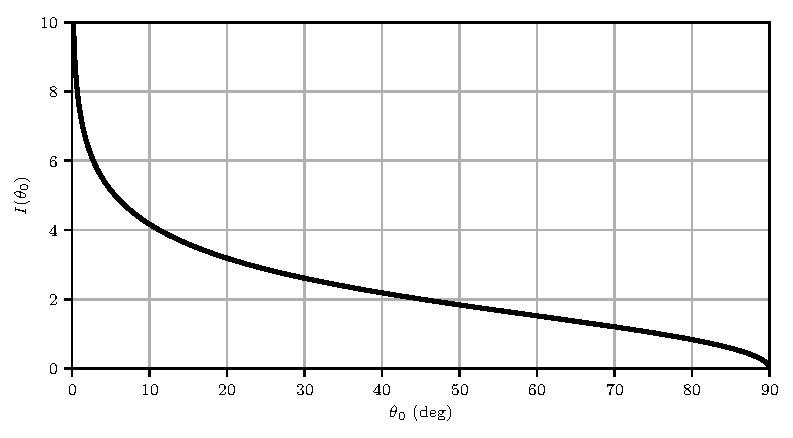
\includegraphics[scale=1]{meca/fonction_I.pdf}
            \vspace{-1em}
            \caption{Graphe de la fonction $I(\theta_0)$.}
        \end{figure}
\end{itemize}

$$\text{En }\theta_0 \rightarrow 0^+, \qquad I(\theta_0) \simeq - \sqrt{2}\ln(\theta_0/\pi).$$
\end{exercise}